% Manuscript B -- IEEE Access (Research Article), on the official IEEE Access LaTeX template
% (ieeeaccess.cls and its fonts and logos, downloaded through the IEEE Template Selector; pristine copy in ieee-template/).
\documentclass{ieeeaccess}
\usepackage{cite}
\usepackage{amsmath,amssymb,amsfonts}
\usepackage{graphicx}
\usepackage{textcomp}
\usepackage{booktabs}
\usepackage{array}
\usepackage{xurl}
\usepackage{xcolor}

\usepackage{bm}
\makeatletter
\AtBeginDocument{\DeclareMathVersion{bold}
\SetSymbolFont{operators}{bold}{T1}{times}{b}{n}
\SetSymbolFont{NewLetters}{bold}{T1}{times}{b}{it}
\SetMathAlphabet{\mathrm}{bold}{T1}{times}{b}{n}
\SetMathAlphabet{\mathit}{bold}{T1}{times}{b}{it}
\SetMathAlphabet{\mathbf}{bold}{T1}{times}{b}{n}
\SetMathAlphabet{\mathtt}{bold}{OT1}{pcr}{b}{n}
\SetSymbolFont{symbols}{bold}{OMS}{cmsy}{b}{n}
\renewcommand\boldmath{\@nomath\boldmath\mathversion{bold}}}
\makeatother

\definecolor{authc}{HTML}{EB6834}
\definecolor{payc}{HTML}{2A78D6}

\newtheorem{proposition}{Proposition}
\newcommand{\cpr}{C-PR}
\newcommand{\spr}{S-PR}
\newcommand{\sha}[1]{\texttt{\footnotesize #1}}

\hyphenation{Page-Rank Endorse-Rank Arbi-trum}

\begin{document}
\history{Date of publication xxxx 00, 0000, date of current version xxxx 00, 0000.}
\doi{10.1109/ACCESS.2024.0429000}

\title{Coupling Authorization and Payment Layers in a PageRank Walk: A Pre-Specified, Hash-Gated Out-of-Window Test on an Ethereum Rollup}
\author{\uppercase{Taehong Kwon}\authorrefmark{1},
\uppercase{Ernest Mnkandla}\authorrefmark{1},
\uppercase{Donatien Koulla Moulla}\authorrefmark{2}, AND
\uppercase{David Sena Attipoe}\authorrefmark{2}}

\address[1]{School of Computing, College of Science, Engineering and Technology, University of South Africa, Johannesburg, South Africa (e-mail: thkwon@enu-tech.co.kr)}
\address[2]{Centre for Augmented Intelligence and Data Science (CAIDS), School of Computing, University of South Africa, Johannesburg, South Africa}
\tfootnote{This research received no external funding.}

\markboth
{Kwon \headeretal: Coupling Authorization and Payment Layers in a PageRank Walk}
{Kwon \headeretal: Coupling Authorization and Payment Layers in a PageRank Walk}

\corresp{Corresponding author: Taehong Kwon (e-mail: thkwon@enu-tech.co.kr).}

\begin{abstract}
Blockchain wallet reputation is usually computed from token payments, yet the same addresses are linked by allowances, through which an owner authorizes a spender to move its tokens. We treat payments and authorizations as two layers of one network and test whether one random walk mixing them at every wallet, weighting edges by raw token amounts, ranks better than the payment walk alone. The data are one-hop networks around 5,521 traders of a derivatives exchange on the Arbitrum One rollup. Most outcomes count the new approvals or payments that the addresses these traders approve, mostly contracts, later receive from them; one is the traders' later share of position closes without liquidation. Two decision rules were fixed in advance: the first, by our dated plan, before any coupled score existed; the second before we extracted its evaluation logs, through a version-controlled commit that the extraction code checks. The coupled walk met neither rule. In the registered window it ranked later approvals better than the payment walk (rank-correlation difference 0.179, 95\% interval 0.132 to 0.225), but on later payers its difference of $-$0.011 ($-$0.025 to 0.003) could not be kept above the margin of $-$0.02, and it trailed the published payment-based method by 0.073. Each layer's raw count beat every walk on that layer's arrivals. With bounded or binary weights the payer contrast fell on either side of the margin. Eleven colluding addresses can lift one of them to 7.7 times the highest bounded-weight authorization score of any sampled trader.
\end{abstract}

\begin{keywords}
Blockchain, decentralized finance, multilayer networks, negative results, PageRank, preregistration, reputation systems, Sybil attacks, token allowances.
\end{keywords}

\titlepgskip=-21pt

\maketitle

% =====================================================================
\section{Introduction}
\label{sec:intro}

\IEEEPARstart{L}{enders} and margin venues in decentralized finance (DeFi) deal with counterparties that are known only by an address \cite{Schar2021}. They rely on over-collateralization and automatic liquidation in place of credit histories \cite{Gudgeon2020Crisis,Werner2022SoK,Perez2021Liquidations}, and a line of research tries to recover some of the missing information from the public ledger. Most of it ranks addresses on a graph of token transfers. Do and Do read PageRank and HodgeRank on Ethereum transactions as a measure of social credit \cite{Do2023PageRank}; Adaptive Weighted PageRank (AWP) weights every transfer by its value and age and restarts the walk at recently active senders \cite{Do2023AWP}; RiskProp propagates account risk through the transaction network \cite{Lin2025RiskProp}. Surveys of blockchain reputation systems find the same reliance on payment volume or on explicit ratings \cite{Bellini2020}. Anyone can recompute such scores from public events, which answers part of the worry that decentralized credit scoring turns into a black box \cite{Packin2024}.

A transfer records a payment. The ledger also records a second relation among the same addresses. Under the ERC-20 (Ethereum Request for Comments 20) token interface an owner calls \texttt{approve} to let a spender draw up to a stated amount of its tokens, and the \texttt{permit} function of Ethereum Improvement Proposal (EIP) 2612 sets the same allowance from an off-chain signature \cite{EIP20,EIP2612}. An allowance moves no funds. It grants a capability that the spender may exercise later and that the owner may raise, lower or revoke, and many allowances are unlimited \cite{Wang2022Penny}. Allowances are far rarer than transfers and point mostly from ordinary wallets to the routers, vaults and trading contracts those wallets use. Payments and authorizations thus form two layers over one set of nodes, the setting of multilayer ranking \cite{Halu2013,DeDomenico2015}.

We ask whether one random walk over both layers ranks addresses better than a walk over either layer alone, and in particular whether adding authorization edges improves on a walk over payments. The registered comparator is our own raw-amount payment walk, which is the end point of the coupled family; AWP, the published payment-based method, is the comparator of a registered sensitivity analysis. On our data the payment layer has about nine times as many edges as the authorization layer, so a walk that mixes the two node by node may simply follow the denser layer. We define a coupled PageRank (\cpr{}) that blends the two transition rows of each wallet with a fixed weight $\lambda$ on the authorization layer, and an ablation, endorsement-seeded PageRank (\spr{}), that walks the payment layer but draws its restarts from the authorization walk, as TrustRank draws its restarts from a vetted seed set \cite{Gyongyi2004TrustRank}.

The evaluation looks forward in time. Scores are frozen at a date and judged by their Kendall rank correlation \cite{Kendall1938} with outcomes that arrive afterwards. The data are one-hop networks around a fixed sample of traders, and the extraction keeps only events with a sampled trader at one end. Two of the three outcomes therefore measure future attachment inside a trader-centered ego network: which addresses, most of them contracts, the sampled traders newly approve or newly pay. We read attachment as a reputation proxy only in a narrow sense, since an approval entrusts funds to the spender and a payment relies on its recipient. The third outcome, the traders' later share of position closes that escaped liquidation, is the one closest to counterparty risk.

Two decision rules were fixed in advance. The first was written in a dated plan after the spring labels were known but before any coupled score was computed; it entered version control only later, so its timing rests on that plan. The second, a three-part comparison of \cpr{} with its payment layer, was committed to our repository before the logs of its evaluation window were extracted, and the extraction script refuses to query unless the committed registration files are unmodified and marked as registered. Both rules failed. We report them as failed, give the commit identifiers and file hashes that let a reader check the second, and add exploratory analyses, clearly marked, that ask whether the failure belongs to the coupling or to the way the operator weights its edges.

The contributions are the following.
\begin{enumerate}
\item A two-layer model of address reputation with a coupled walk, a seeded ablation and two analytic remarks: for $\lambda$ strictly between 0 and 1 the weight acts only through wallets with out-edges in both layers, and on a one-hop sample the authorization walk reduces to an owner-normalized in-strength. Empirically the coupled ranking changes mainly at the two end points of the family.
\item A pre-specified protocol for ranking experiments on ledger data, with a hash-checked extraction step, together with the weaknesses we found in it: a margin set from precision rather than relevance, a ``no worse'' criterion that rewards imprecision, and a registration that outsiders can date only through repository and server timestamps.
\item A negative result on the Arbitrum One rollup. \cpr{} met neither rule. Its gain over the payment walk on later approvals held again in a window whose sample was fixed before its outcomes, and, as a secondary result outside the failed rule, it ranked later liquidation-free trading slightly better; but a loss on later transfer senders larger than the registered margin could not be ruled out, and against AWP the loss exceeded the margin. In both windows the raw degree of each layer ranked that layer's later arrivals better than every walk.
\item A calibration of known link-farm results to the authorization layer under uniform restarts. A star of ten farm addresses lifts its target to 7.7 times the highest bounded-weight authorization score among the sampled traders, though not near the top contracts; the same farm gains far less on the payment walks.
\end{enumerate}

A companion manuscript \cite{KwonA2026} compares the two edge types as separate scores, sets each against its raw degree and studies trader outcomes built from neither edge type. We draw on it for the data pipeline and for the closed form of the authorization walk; this paper concerns the coupling operator, its pre-specified test and the manipulability of the authorization layer. Section~\ref{sec:related} reviews related work, Section~\ref{sec:model} defines the model, Section~\ref{sec:protocol} states the rules and their record, Section~\ref{sec:data} describes data and measurement, Section~\ref{sec:results} reports the results, Section~\ref{sec:sybil} calibrates farm attacks, Section~\ref{sec:threats} discusses threats to validity, Section~\ref{sec:implications} draws implications for lending and margin protocols, and Section~\ref{sec:conclusion} concludes. Appendix~\ref{app:explore} collects the exploratory checks.

% =====================================================================
\section{Related Work}
\label{sec:related}

\subsection{Reputation From Ledger Graphs}
PageRank ranks the nodes of a directed graph by the stationary distribution of a damped random walk \cite{Page1998,Langville2006}. Hyperlink-Induced Topic Search (HITS) separates hubs from authorities \cite{Kleinberg1999}, and EigenTrust normalizes local trust values so that peers in a file-sharing network cannot inflate their own standing \cite{Kamvar2003}. On public ledgers these ideas have been applied almost entirely to transfers. Besides the methods named above \cite{Do2023PageRank,Do2023AWP,Lin2025RiskProp}, network embeddings of transaction graphs detect phishing accounts better than per-account features \cite{Wu2022Phishers}, and a survey of knowledge discovery in cryptocurrency transactions lists degree- and value-based centralities as the usual wallet descriptors \cite{Liu2021Knowledge}. Approvals appear in earlier work in two roles: as a clustering heuristic that links addresses of one entity \cite{Victor2020Clustering}, and as a security risk when unlimited \cite{Wang2022Penny}. Deployed tooling such as Human Passport scores the holder of an address from weighted credentials and does not rank relations between addresses \cite{HumanPassport}. The companion study \cite{KwonA2026} uses the latest allowance as the edge of a ranking; the present paper combines that edge with the payment edge in one walk.

\subsection{Multilayer and Personalized Ranking}
Multiplex PageRank lets the centrality a node earns in one layer bias the walk in another \cite{Halu2013}, and the interconnected-multilayer framework of De Domenico \emph{et al.} lets a walker move inside layers and switch between them, ranking nodes by their versatility across layers \cite{DeDomenico2015}. Topic-sensitive and personalized PageRank change the teleportation vector instead of the transition matrix \cite{Haveliwala2003,Jeh2003}, and TrustRank confines teleportation to a hand-checked seed set to demote web spam \cite{Gyongyi2004TrustRank}. \cpr{} is a special case of the first family: a per-node convex combination of two row-stochastic matrices with one global weight and no copies of a node across layers. \spr{} belongs to the second family. Proposition~\ref{prop:localize} below is a first-order perturbation bound of the standard kind for PageRank \cite{Langville2006}, specialized to this convex combination. What we have not found in the literature is a test of either construction on two on-chain relations among the same addresses, judged by a rule fixed before its evaluation data were extracted.

\subsection{Degree Baselines}
Under preferential attachment new links go disproportionately to nodes that already have many \cite{Barabasi1999}, and measurements of growing networks show the same tendency \cite{Newman2001}. Degree-based scores are therefore standard baselines in link prediction \cite{LibenNowell2007}, including on Ethereum transaction networks \cite{Lin2022Tracking}, and on graphs with weak degree correlations PageRank is on average proportional to in-degree \cite{Fortunato2008}. A claim that a walk adds information should thus be tested against the raw degree it smooths, and we set every walk against it.

\subsection{Manipulation and Sybil Resistance}
Where identities are free, one actor can appear as many \cite{Douceur2002}. Gy\"{o}ngyi and Garcia-Molina derive the link farms and alliances that raise a target's PageRank the most \cite{Gyongyi2005Alliances}. Cheng and Friedman show that no symmetric reputation function, PageRank included, is Sybil-proof, whereas some asymmetric functions computed from flows or paths out of a trusted source are \cite{Cheng2005}. Section~\ref{sec:sybil} applies these results to the authorization layer; it calibrates them rather than deriving new ones. On ledgers, wash trading inflates payment activity \cite{Victor2021Wash,Cong2023Wash}, proof-of-personhood schemes trade Sybil resistance against privacy and self-sovereignty \cite{Siddarth2020}, and a recent security review names credential farming as the main residual weakness of Human Passport \cite{Bordeianu2026}.

\subsection{Pre-Specified Analyses}
Preregistration separates the analyses that test a hypothesis from those that generate one, and it can be applied to data that already exist, provided the analysts have not yet examined the outcomes \cite{Nosek2018}. With observational ledger data the events of a test window exist on chain from the moment they occur, so the strongest practical guarantee is that the analysts had not extracted them when the rule was fixed. Construct-validity theory adds a caution that matters below: a score should agree with checks of what it was designed to track, so such agreement is not independent evidence \cite{Cronbach1955}.

% =====================================================================
\section{Model}
\label{sec:model}

\subsection{Two Layers on One Set of Addresses}
Let $V=V_A\cup V_T$ be the set of addresses in either layer (Fig.~\ref{fig:layers}). We use \emph{authorization} for the layer, its edges and its walk, \emph{approval} for the event that creates an edge, and \emph{allowance} for the approved amount; likewise \emph{payment} for the second layer and \emph{transfer} for its events. An authorization edge $u\to v$ exists when the latest in-window \texttt{Approval} event from owner $u$ to spender $v$ carries a positive value on at least one token. The window starts on 1~December~2025 and ends at the freeze date, and a latest value of zero removes the pair. This is what the pipeline measures, and it differs from the allowance in force in five ways: (i) allowances granted before the window and not re-emitted inside it are invisible, so a later approval of such a pair looks new; (ii) a finite allowance that \texttt{transferFrom} has since drawn down keeps its approved value, because a token need not emit an \texttt{Approval} event when an allowance is spent; (iii) an owner who approves an allowance manager such as Uniswap's Permit2 appears with an edge to that manager only; (iv) payments in native ether emit no log and are missing from the payment layer; and (v) ERC-721 tokens emit \texttt{Approval} and \texttt{Transfer} logs under the same signatures. Section~\ref{sec:data} states how the extraction treats (v), and Section~\ref{sec:threats} quantifies (i), (iii) and (v). A payment edge $u\to v$ exists when $u$ sent $v$ at least one token transfer with a positive amount in the window. The operator studied here weights both layers by raw amounts:
\begin{equation}
\tilde w_A(u,v)=\sum_{\text{token}} a^{\star}(u,v,\text{token}),
\label{eq:layerA}
\end{equation}
\begin{equation}
\tilde w_T(u,v)=\sum_{e:\,u\to v} x_e\,\sigma(\Delta t_e),
\label{eq:layerT}
\end{equation}
where $a^{\star}$ is the latest allowance in token base units, $x_e$ the amount of transfer $e$ in base units, and $\sigma(\Delta t)=1/(1+\exp(k(\Delta t-t_0)))$ a logistic discount on the age $\Delta t$ in days, the form used by AWP \cite{Do2023AWP}; that paper fixes no parameter values, and $k=0.01$ and $t_0=180$ are our choices. Ages are measured back from the freeze date. The authorization layer is not discounted. Write $o_A(u)$ and $o_T(u)$ for the out-strengths and $P_A$, $P_T$ for the row-normalized matrices, whose rows are zero where a node has no out-edge in that layer.

% Fig. 1: schematic of the two layers, the coupled row and the seeded restart.
\begin{figure}[!t]
\centering
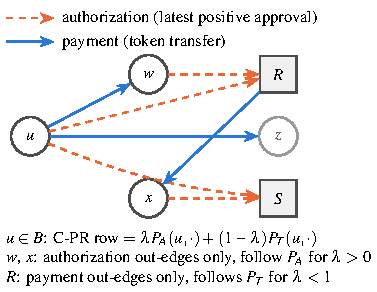
\includegraphics[width=\columnwidth]{figures/fig_layers.pdf}
\caption{The two layers on one set of addresses (schematic). Circles are sampled traders and squares are contracts such as routers and vaults; $z$ is an address outside the sample, present only because a sampled trader paid it. Only $u$ has out-edges in both layers, so only its row depends on $\lambda$ for $0<\lambda<1$. At $\lambda=1$ the payment edges and $z$ are dropped, so $R$ becomes dangling; at $\lambda=0$ the authorization edges are dropped, so $w$ and $x$ become dangling and $S$ leaves the graph. \spr{} walks the solid edges only and restarts each jump in proportion to the authorization walk's score.}
\label{fig:layers}
\end{figure}


\subsection{PageRank With a Restart Distribution}
Every score below is the fixed point of
\begin{equation}
\mathbf r^{(t+1)}=(1-d)\,\boldsymbol\pi+d\,P^{\top}\mathbf r^{(t)}+d\,\bigl(\mathbf 1_{\mathrm{dang}}^{\top}\mathbf r^{(t)}\bigr)\,\boldsymbol\pi,
\label{eq:pr}
\end{equation}
where $P$ is the transition matrix, $\boldsymbol\pi$ the restart distribution, and $\mathbf 1_{\mathrm{dang}}$ the indicator of nodes with an all-zero row, whose mass is sent back through $\boldsymbol\pi$. We use $d=0.85$, start from the uniform vector, and stop when the $\ell_1$ change falls below $10^{-8}$ or after 300 iterations.

\subsection{Coupled PageRank}
\cpr{} mixes the two rows of each node, renormalizing over the layers in which the node has out-edges:
\begin{equation}
P^{(\lambda)}_{u\cdot}=\alpha_A(u)\,P_{A,u\cdot}+\alpha_T(u)\,P_{T,u\cdot},
\label{eq:cpr}
\end{equation}
\begin{equation}
\alpha_A(u)=\frac{\lambda\,\mathbf 1[o_A(u)>0]}{D_\lambda(u)},\quad
\alpha_T(u)=\frac{(1-\lambda)\,\mathbf 1[o_T(u)>0]}{D_\lambda(u)},
\label{eq:alpha}
\end{equation}
with $D_\lambda(u)=\lambda\,\mathbf 1[o_A(u)>0]+(1-\lambda)\,\mathbf 1[o_T(u)>0]$. A node with out-edges in one layer follows that layer with weight one, and a node with none in either is dangling. Restarts are uniform. The primary setting $\lambda=0.5$ and the sensitivity values $0.25$ and $0.75$ were fixed with the first rule (Section~\ref{sec:protocol}).

At $\lambda=1$ the payment layer is dropped together with the nodes only it contains, and the operator becomes PageRank on the authorization layer alone; at $\lambda=0$ it becomes PageRank on the payment layer alone. We call these the authorization walk and the payment walk; they are the comparators of both rules. The family is discontinuous at both ends. For every $\lambda$ strictly between 0 and 1, a node whose out-edges are all payments follows the payment layer, whereas at $\lambda=1$ the same node is dangling or absent. Symmetrically, a node whose out-edges are all authorizations follows the authorization layer at every interior $\lambda$ but is dangling or absent at $\lambda=0$. Unit tests on a fixture graph check that each end point reproduces its single-layer walk.

\subsection{Seeded Ablation}
\spr{} keeps the payment walk and replaces its uniform restart vector by the authorization walk's score $\mathbf r_A$, restricted to $V_T$ and renormalized:
\begin{equation}
\pi_u=\frac{r_{A,u}}{\sum_{v\in V_T} r_{A,v}},\qquad u\in V_T,
\label{eq:spr}
\end{equation}
with $r_{A,u}=0$ for $u\notin V_A$ and a uniform fallback if the denominator vanishes. Authorization then decides where the walker lands after a jump, and payments decide where it goes between jumps. Comparing \spr{} with \cpr{} separates the authorization edge as a route from the authorization edge as a seed.

\subsection{Reference Scores}
Two published or companion scores and two counts serve as references. AWP \cite{Do2023AWP} walks the payment layer with weights $\sigma(\Delta t_e)V(x_e)$ summed over transfers, where $V(z)=2/(1+e^{-bz})-1$ is a bounded value transform, and restarts at each address in proportion to its recent sending activity. The paper fixes neither $b$ nor the unit of $z$; we apply $b=1$ to base units, in which $V(z)$ is within $10^{-4}$ of one for any amount of ten units or more, so this reading of AWP counts recency-weighted transfers. Other units would give another variant, and we use the name AWP for ours. EndorseRank \cite{KwonA2026} walks the authorization layer with the same bounded weights and uniform restarts. Both reference walks therefore count events, whereas \cpr{} lets amounts matter. The counts are the in-approve degree, the number of distinct owners holding a positive latest allowance to the address, and the transfer in-degree, the number of distinct addresses other than itself that sent it a transfer, both taken at the freeze.

\subsection{Where the Weight Acts}
Let $B=\{u: o_A(u)>0 \text{ and } o_T(u)>0\}$ be the set of nodes with out-edges in both layers.

\begin{proposition}
\label{prop:localize}
For $\lambda\in(0,1)$ and uniform $\boldsymbol\pi$, the rows of $P^{(\lambda)}$ outside $B$ do not depend on $\lambda$, and the derivative $\mathbf r'(\lambda)$ of the stationary vector of (\ref{eq:pr}) with respect to $\lambda$ satisfies
\begin{equation}
\mathbf r'(\lambda)=d\,\bigl(I-d\,G_\lambda^{\top}\bigr)^{-1}\sum_{u\in B} r_u\bigl(\mathbf p_{A,u}-\mathbf p_{T,u}\bigr),
\label{eq:sens}
\end{equation}
where $\mathbf p_{A,u}$ and $\mathbf p_{T,u}$ are the transposed rows of $P_A$ and $P_T$ and $G_\lambda$ is $P^{(\lambda)}$ with each dangling row replaced by $\boldsymbol\pi^{\top}$. Hence $\|\mathbf r'(\lambda)\|_1\le 2d\,r(B)/(1-d)$ with $r(B)=\sum_{u\in B}r_u$.
\end{proposition}

\begin{IEEEproof}
Outside $B$ one indicator in (\ref{eq:alpha}) is zero, so the row is a single layer's row or zero whatever $\lambda$ is, and the dangling set does not change on $(0,1)$. For $u\in B$, $D_\lambda(u)=1$ and the row is $\lambda P_{A,u\cdot}+(1-\lambda)P_{T,u\cdot}$, whose derivative is $P_{A,u\cdot}-P_{T,u\cdot}$. Because $\mathbf r$ sums to one, (\ref{eq:pr}) can be written $\mathbf r=(1-d)\boldsymbol\pi+d\,G_\lambda^{\top}\mathbf r$; differentiating gives (\ref{eq:sens}). The matrix $G_\lambda^{\top}$ is column-stochastic, so $\|(I-dG_\lambda^{\top})^{-1}\|_1\le 1/(1-d)$, and each difference of two probability rows has $\ell_1$ norm at most 2.
\end{IEEEproof}

The proposition says where the weight can act; it does not say that the action is small. On our spender graphs $B$ is large: at the end of the window it holds 4,461 of the 7,929 nodes, and $r(B)$ is 0.44 at $\lambda=0.5$, so the bound is near 5 per unit of $\lambda$, weaker than the trivial bound of 2 on the $\ell_1$ distance between two distributions. Section~\ref{sec:sweep} reports how far the stationary vector and the ranking actually move.

\subsection{The Authorization Walk on a One-Hop Sample}
Our graphs keep only events with a sampled trader at one end, so almost every node of the authorization layer either only grants approvals (a pure owner) or only receives them (a pure spender). The companion study derives a closed form for this structure \cite{KwonA2026}; we restate it with its proof.

\begin{proposition}
\label{prop:closed}
Under (\ref{eq:pr}) with uniform $\boldsymbol\pi$, every node without in-edges has the same score $c$, and a node $v$ whose in-neighbors all lack in-edges scores $r_v=c\,(1+d\,\delta(v))$, where $\delta(v)=\sum_u w(u,v)/o(u)$ is its owner-normalized in-strength.
\end{proposition}

\begin{IEEEproof}
With uniform restarts and dangling mass $r_D$, (\ref{eq:pr}) reads $r_v=(1-d+d\,r_D)/|V|+d\sum_u r_u\,w(u,v)/o(u)$. A node without in-edges receives only the first term, which we call $c$. If every in-neighbor $u$ of $v$ lacks in-edges, then $r_u=c$, and substituting gives $r_v=c+d\,c\,\delta(v)$.
\end{IEEEproof}

The statement holds for any edge weights, so it covers both EndorseRank and \cpr{} at $\lambda=1$, each with its own $\delta$. With bounded weights it fits 96.4\% and 97.4\% of the spenders to within 1\% at the two freeze dates \cite{KwonA2026}. With raw amounts an owner's unlimited approvals share its whole row and its finite ones receive almost nothing. Either way the authorization walk on this sample is a reweighted count of approving owners, with depth one, and \cpr{} inherits that limit wherever it follows the authorization layer.

\subsection{Cost}
On the trader graph at the end of the window (151,814 edges on 31,242 nodes), one \cpr{} solve took 5.67\,s, against 5.03\,s for AWP and 0.55\,s for EndorseRank (mean of five timed runs after a warm-up on four cores of an Intel Xeon at 2.8\,GHz with 15\,GB of memory, Python 3.11, NumPy 2.4, SciPy 1.17); \cpr{} thus costs more than AWP, which walks the same transfer edges, and the payment walk itself was not timed.

% =====================================================================
\section{Pre-Specified Rules and Their Record}
\label{sec:protocol}

Table~\ref{tab:timeline} lists the commitments in the order in which they were made, the record that dates each one, and what was known at each point. Three features of this history matter for interpretation. First, Rule~A was fixed after the spring labels and the spring results of the two single-layer walks were known; only the coupled scores were unseen, and that ordering is documented by a dated plan rather than by a commit. Second, the comparison that motivated Rule~B was noticed after the spring results were in, so the spring evidence for it is exploratory. Third, when Rule~B's trader label was chosen we knew its spring prevalence (923 of 1,860 traders in the freeze-date graph had at least one liquidation) and its same-window coefficients for the two single-layer walks (0.075 for the authorization walk and 0.083 for the payment walk), but never its out-of-window value for any score.

% Table 1: order of commitments and their records. Sources: the commit history of the
% authors' repository phd_works (GitHub API: commit, push-event and pull-request times),
% the registration plan docs/fresh_holdout_2026q3_plan.md, the extraction manifest and
% evaluation summary of the registered replication, and thesis Sections sub:coupled-graph,
% sec:holdout-protocol, sub:fresh-holdout and the reproducibility appendix.
\begin{table*}[!t]
\centering
\caption{Order of Commitments, the Record of Each, and What Was Known When It Was Made (Dates in 2026, Times in UTC)}
\label{tab:timeline}
\footnotesize
\setlength{\tabcolsep}{3pt}
\renewcommand{\arraystretch}{1.08}
\begin{tabular}{@{}>{\raggedright\arraybackslash}p{0.085\textwidth}>{\raggedright\arraybackslash}p{0.355\textwidth}>{\raggedright\arraybackslash}p{0.285\textwidth}>{\raggedright\arraybackslash}p{0.235\textwidth}@{}}
\toprule
When & Commitment or event & Record & Already known \\
\midrule
29 Aug & Exploratory spring run on the trader cohort with three trading-success labels; only the two single-layer walks were scored, with no liquidation label and no coupled score & Disclosed in the Rule~B plan & Spring labels \\
14 Sep & Coupled operator, $\lambda\in\{0.25,0.5,0.75\}$ and Rule~A written in a dated plan & Plan dated 14 Sep; first committed, with the configuration, in \texttt{0097fdb} on 28 Sep, the commit that also holds the first coupled spring results & Spring labels; spring results of both single-layer walks; the 29 Aug run \\
14--28 Sep & Coupled spring scores computed and Rule~A evaluated & Summary file records a run at 14 Sep, 08:54; first committed in \texttt{0097fdb} & --- \\
28 Sep, 08:43 & Rule~B (F1--F3, with F4--F6 to be reported), its window and its trader label written in a configuration file (status ``draft'') and a plan & \texttt{0097fdb}; push recorded by GitHub at 22:07:54 & All spring results, including the exploratory gain; the spring prevalence and same-window coefficients of the trader label (see Section~\ref{sec:protocol}) \\
1 Oct, 12:50 & Sensitivity analyses S1 and S2 added to the configuration and the plan & \texttt{f54d10c}, the plan's last change & Spring scores of AWP \\
1 Oct, 13:28 & Status set to ``registered'' & \texttt{4085ab9}; push recorded by GitHub at 13:28:45; merged at 13:33:45 (\texttt{f701400}) & No June--August log \\
1 Oct, 14:05--14:07 & Dry run and nine extraction jobs; manifest records both file hashes and no override & Manifest; extracts in \texttt{d6d26c4} (pushed 14:17:32) & --- \\
1 Oct, 14:23 & Registered evaluation, code as of \texttt{4085ab9} & Summary in \texttt{1462d76} (pushed 14:28:44), byte-identical today & --- \\
2 Oct & EndorseRank scored on the registered cohorts outside the rule; code revised for the reference scores (\texttt{ce50659}); spring check rerun with identical values & Registered summary not regenerated & Registered results \\
9 Oct & Plan of the post hoc trader comparison, source of the decomposition rows of Table~\ref{tab:contrasts} & \texttt{20e250f} (thesis repository) & Registered labels and single-score coefficients \\
9 Oct & Exploratory diagnostics of Appendix~\ref{app:explore} & This paper's supplement & Every result above \\
\bottomrule
\end{tabular}

\vspace{2pt}
\parbox{\textwidth}{\footnotesize Full commit identifiers and file hashes are listed in Section~\ref{sec:gate}. Spring scores use 90 days of history (1 December 2025 to 28 February 2026); registered scores use 182 days (1 December 2025 to 31 May 2026).}
\end{table*}


\subsection{Rule A (Dated 14 September 2026)}
Rule~A asked whether \cpr{} beats both layers walked alone. Its primary part used the spring holdout: at $\lambda=0.5$, \cpr{} should do no worse than the authorization walk on new approval pairs, meaning that the 95\% interval of $\Delta\tau=\tau_{\text{\cpr{}}}-\tau_{\lambda=1}$ contains zero or lies above it, and should beat the payment walk on new transfer senders, meaning that the interval of $\tau_{\text{\cpr{}}}-\tau_{\lambda=0}$ lies above zero. Its secondary part used same-window checks on the sampled traders. \cpr{}'s point estimate had to lie inside the 95\% interval of the leading layer on the payment-check family and on the authorization-check family, and \cpr{} had to exceed both layers on a family of three activity-stability checks (the share of distinct inbound counterparties, tenure and active months). No $\lambda$ was to be tuned after labels were seen.

The rule is recorded in a plan dated 14 September, which states that its criteria were fixed before any of the new numbers were computed. The plan and the configuration that encodes the rule entered version control together on 28 September, in commit \sha{0097fdb}, which also holds the first coupled spring results; the summary file of those results records a run time of 14 September, 08:54~UTC. The repository therefore does not show that the rule preceded the coupled scores; that rests on the dated plan and on our account. Two criteria of the rule are weak by design. ``No worse'' as defined rewards imprecision, since a wider interval contains zero more easily, and the secondary part compares a point estimate with another score's marginal interval rather than using a paired contrast. Anyone reusing the protocol should replace the first by a non-inferiority margin and the second by paired contrasts.

\subsection{Rule B (Written 28 September, Registered 1 October 2026)}
Rule~B asked whether \cpr{} improves on the payment walk, $\Delta\tau=\tau_{\text{\cpr{}}}-\tau_{\lambda=0}$, in a window frozen on 31 May 2026 with labels counted from 1 June to 31 August 2026:
\begin{itemize}
\item F1 (spenders; new approval pairs), superiority: the whole 95\% interval of $\Delta\tau$ must be positive;
\item F2 (spenders; new transfer senders), non-inferiority: the interval must not reach $-0.02$ or below;
\item F3 (traders; liquidation-free close rate), non-inferiority with the same margin of $-0.02$.
\end{itemize}
All three had to hold. Because the decision is an intersection of three conditions, testing each at the 5\% level keeps the probability of a false claim of improvement at or below 5\% without a multiplicity correction (the intersection--union principle). The margin $0.02$ is the half-width of the spring interval for the contrast that F2 repeats. It measures the precision of the spring estimate, not a difference judged to matter in practice, and it would have shrunk with more data. Computed afterwards from the bootstrap standard deviations of that contrast under a normal approximation, F2 had a 0.51 chance of passing at spring precision if the true difference were zero and 0.77 if it equalled the spring estimate of $+0.007$; at the precision reached in the registered window the chances were 0.78 and 0.96. The plan also recorded a weakness of F3 in advance: it could pass with both coefficients near zero if neither walk predicted liquidation, so both coefficients are reported beside the verdict.

Three further contrasts were to be reported in a fixed order outside the decision: F4, superiority of \cpr{} over the payment walk on the liquidation-free close rate; F5, superiority over the authorization walk on that label; and F6, the primary part of Rule~A rerun on the new window. ``Fixed order'' meant only the order of reporting; there was no gatekeeping, so F4 to F6 are nominal results with unadjusted 95\% intervals. Two sensitivity analyses were added on 1 October, after AWP had been scored on spring data and before extraction: S1 repeats F1 to F4 with AWP as the comparator, and S2 repeats F1 to F6 with sampled wallets absent from a graph kept as isolated nodes rather than scored zero. Neither enters the decision, and their verdicts are nominal as well. Solver, $\lambda$, query text, wallet filter, exchange-event decoder and bootstrap (400 paired resamples, seed 42) were those of the spring analysis. The score window was not: spring scores use 90 days of history and registered scores 182 days, since both start on 1 December 2025.

\subsection{Gate on Extraction}
\label{sec:gate}
The configuration and the plan were committed with a status field, and the status was set to ``registered'' on 1 October at 13:28:09~UTC. Table~\ref{tab:ids} gives the full identifiers of that commit and of its neighbors, and the SHA-256 hashes of both files. GitHub, which hosts the repository, recorded the push of the registration commit at 13:28:45 and the merge of its pull request at 13:33:45; these server-side times are not set by the committer. Before it queries anything, the extraction script checks that both files are tracked, unmodified and marked as registered; it writes their SHA-256 hashes into its manifest, and the evaluation copies them into its summary. The recorded hashes were computed on the authors' checkout, which stores the files with CRLF line endings; a checkout with LF line endings gives the second pair in Table~\ref{tab:ids}. A testing override exists; it writes a flag into the manifest when used, and the manifest has none. The manifest dates the dry run at 14:05:25, and the nine monthly BigQuery jobs finished between 14:05:37 and 14:07:27. The evaluation summary was produced at 14:23 with the code as committed at registration, since the two commits of that hour add only data and the summary, and the summary file is byte-identical in the current revision. Before any new coefficient was computed, the evaluation code was run on the spring window and returned, to the last digit, the sixteen spring coefficients of the eight scores common to both analyses, together with the Rule~A contrasts. On 2 October the code that computes the reference scores was revised (\sha{ce50659}); the registered summary was not regenerated, and a rerun of the spring check gave identical values.

% Table: identifiers of the registration record. Sources: GitHub API for the authors'
% repository phd_works (commits, push events, pull request 1) and the extraction
% manifest of the registered replication; LF hashes recomputed from the files.
\begin{table}[!t]
\centering
\caption{Identifiers of the Registration and Extraction Record (1 October 2026 Unless Stated, Times in UTC)}
\label{tab:ids}
\footnotesize
\setlength{\tabcolsep}{0pt}
\begin{tabular}{@{}>{\raggedright\arraybackslash}p{\columnwidth}@{}}
\toprule
Rule files first committed, 28 Sep 08:43 (pushed 22:07:54)\\
\quad\sha{0097fdb2a51b82f96c63a47fe08e7b2b8f120410}\\
Last change of the plan, 12:50:40\\
\quad\sha{f54d10c577070fc9a5a0f0f22826dde5c2a8321f}\\
Status set to registered, 13:28:09 (pushed 13:28:45)\\
\quad\sha{4085ab919e7fdfc0b444d25a6c7f217b663272b5}\\
Merge of the registration pull request, 13:33:45\\
\quad\sha{f701400cd893994dbf5b5f4c8b5f0051f6dcc915}\\
Extracts and manifest committed (pushed 14:17:32)\\
\quad\sha{d6d26c4ae526aa5eb91d7306cd495e919c27d675}\\
Evaluation summary committed (pushed 14:28:44)\\
\quad\sha{1462d76fd7b9d70e44b9b2e851bcc33c8d150e2e}\\
\midrule
SHA-256 of the configuration, CRLF line endings (as recorded)\\
\quad\sha{9777f3098d4e5e6d7bb2e8fda590b171}\\
\quad\sha{c549e643731818a8b6eb079e853609ff}\\
SHA-256 of the plan, CRLF line endings (as recorded)\\
\quad\sha{e1b45e9b20a46e21417c45c84e0fe023}\\
\quad\sha{1207d1b167c3569756ac72381d240a99}\\
SHA-256 of the configuration, LF line endings\\
\quad\sha{6291f423b31c5488ab3a8f1209c09eb0}\\
\quad\sha{9ba9d633f734b7cba39677514a1f36c0}\\
SHA-256 of the plan, LF line endings\\
\quad\sha{845aef23bfc1005ed0048e1ba1b2c25e}\\
\quad\sha{2f87036dc55484d46d3f6089294669cb}\\
\bottomrule
\end{tabular}
\end{table}


The registration is a commit in the authors' own public repository, not an entry in an independent registry (Data Availability). The push and merge times are kept by GitHub rather than by us, so others can check them.

\subsection{What Was Not Registered}
The registered score list did not include EndorseRank. We computed it on the registered cohorts the day after the evaluation, and it serves only as a reference. The spring comparisons of \cpr{} with the payment walk on new approval pairs, with AWP and with EndorseRank were made after the labels were known. The decomposition rows at the foot of Table~\ref{tab:contrasts} come from a post hoc analysis whose plan was committed after the registered labels were known but before any of its contrasts was computed; it uses 2,000 paired resamples. Every analysis in Appendix~\ref{app:explore} was run on 9 October, after all of the above, and is exploratory.

% =====================================================================
\section{Data and Measurement}
\label{sec:data}

\subsection{Sources and Sample}
The companion study describes the pipeline \cite{KwonA2026}; we give here what is needed to reproduce the coupled analysis, and the supplement holds the query files and the analysis script. All logs come from Arbitrum One, an optimistic rollup on Ethereum \cite{Kalodner2018,Thibault2022}, through the public BigQuery table and, for exchange events, from the GMX event emitter, both named below:
\begin{center}
\texttt{\scriptsize bigquery-public-data.goog\_blockchain\_arbitrum\_one\_us.logs}\\[1pt]
\texttt{\footnotesize 0xC8ee91A54287DB53897056e12D9819156D3822Fb}
\end{center}
The base window runs from 1 December 2025 to 31 May 2026. The sample is the 5,521 wallets with at least three position closes on the GMX~V2 perpetual-futures exchange \cite{GMXDocs} in that window; we call them the sampled traders. A close is one \texttt{EventLog1} record of that emitter whose event name is \texttt{PositionDecrease}, so partial closes and liquidations count; a close is a liquidation when its order type is 7 or when it was sent by the exchange's liquidation handler. The sample was fixed from exchange events before any approval or transfer was extracted.

Approval and transfer logs are selected by the ERC-20 event signature in the first topic, at least three topics, and a sampled trader in the second or third topic; the amount is the data field read as an unsigned 256-bit integer. ERC-721 events share the signatures but carry four topics and an empty data field, so they pass this filter with amount zero: they create no authorization edge and no weighted payment edge, but a zero-amount transfer still counts toward the transfer in-degree and the new-sender label. ERC-1155 events use other signatures and are not extracted. Mints from and burns to the zero address are kept as ordinary transfers; self-transfers are kept in the payment layer but excluded from the transfer in-degree and the new-sender label.

\subsection{Graphs}
Each cohort's walks keep the edges with at least one end in that cohort, which adds the cohort's one-hop neighbors as nodes. For the trader cohort this is the whole extracted graph: at the end of the window the authorization layer has 6,442 nodes and 14,727 edges, one of them a self-loop that the closed-form check of the companion study drops, and the payment layer 30,791 nodes and 137,087 edges. For the spender cohort the payment layer holds only transfers into or out of a spender: 31,102 edges at the end of the window and 17,273 at the spring freeze, so \cpr{} walks 7,929 and 5,928 nodes respectively. Wallets of a cohort absent from a walk's graph score zero under that walk (sensitivity S2 changes this). Of the 21,585 latest allowances at the end of the window, 13,055 (60.5\%) are unlimited, recorded as $2^{256}-1\approx1.16\times10^{77}$ base units, and 3,986 of the 4,590 owners hold at least one. In the raw-amount layer such an owner's row is split among its unlimited approvals. Transfer amounts in different tokens are summed in raw units, so tokens with more decimal places weigh more. These are properties of the operator as fixed with Rule~A; both rules were judged on it as specified, and Appendix~\ref{app:explore} reruns the coupling with bounded and with binary weights.

\subsection{Cohorts and Labels}
Spenders are all addresses holding at least one positive latest allowance at the freeze: 1,335 in the spring analysis (freeze 28 February 2026, labels 1 March to 31 May 2026), of which 1,174 held contract code, and 1,964 in the registered window. Their first label counts new approval pairs: owners that gave the spender a positive approval during the label window although the pair was absent from the latest-positive snapshot at the freeze. Their second label counts new transfer senders: addresses other than the spender that sent it a transfer during the label window but had not done so between 1 December 2025 and the freeze. Both labels are counted on events extracted with the same wallet filter, so they record what the sampled traders do: 5,346 of the 5,353 spring approval-pair events and 2,163 of the 2,168 registered ones come from a sampled owner. In the registered window the trader cohort is the 5,151 sampled traders present in the freeze-date graph, and its label is defined for the 1,402 that closed at least three positions from June to August; the spring counterpart, used only in post hoc rows, has 1,860 traders. The label is the liquidation-free close rate, one minus the share of a trader's closes in the label window that ended in liquidation. Forced liquidation is the outcome closest to default in these data \cite{Perez2021Liquidations}, the label is built from neither layer, and as a rate it does not reward trading more. Extraction for June to August yielded 163,553 approval and 1,013,023 transfer logs together with 144,152 exchange closes.

The two windows were not generated in the same way. The sample was selected on closes up to 31 May 2026, a period that contains the spring label window. In the registered window it was fixed before the labels, but in the spring 1,584 sampled traders had fewer than three closes by the spring freeze and qualified for the sample only through closes made inside the spring label window; they generated 3,027 of the 5,353 spring approval-pair events and 1,940 of the 3,107 new-sender events. Appendix~\ref{app:explore} reruns the spring analysis on the sample selected from December to February alone.

\subsection{Statistics}
Every coefficient is the tie-corrected Kendall $\tau_b$ \cite{Kendall1938}, computed with SciPy, with a 95\% percentile interval from a paired wallet bootstrap \cite{Efron1979,DiCiccio1996}. Resample indices are drawn with NumPy's default generator (PCG64) from seed 42, one index vector per resample, and the same matrix of indices serves every score on a label, so each difference between two scores is a paired difference. Every result uses 400 resamples except the post hoc rows, which use 2,000.

% =====================================================================
\section{Results}
\label{sec:results}

\subsection{Same Window: The Mixture Follows the Denser Layer}
\label{sec:res-window}
On the sampled traders over the base window, \cpr{} at $\lambda=0.5$ reaches a family-mean $\tau$ of 0.527 on the payment checks (in-degree and inflow), just below the payment walk at 0.534, a paired gap of $-0.007$ $[-0.009,-0.005]$; AWP reaches 0.612. On the authorization checks (in-approve degree and approved amount) \cpr{} sits at $-0.001$, while the authorization walk reaches 0.355, a gap of $-0.356$ $[-0.388,-0.323]$. Raising $\lambda$ to 0.75 lifts \cpr{} on this family only to 0.006. On the activity-stability checks it scores 0.290, above both the payment walk (0.286) and the authorization walk (0.233), with paired intervals $[0.003,0.006]$ and $[0.043,0.069]$. The secondary part of Rule~A therefore passes on payments and stability and fails on authorization, since $-0.001$ lies far outside the authorization walk's interval $[0.322,0.384]$. \spr{} falls below the layer it borrows from on every family (0.494, 0.116 and 0.220). These same-window checks come from the events that build the graphs, so they show which construct a score tracks and are not external evidence \cite{Cronbach1955}.

\subsection{Spring Holdout: Rule A Fails}
Table~\ref{tab:holdout} gives every score against the later labels, Table~\ref{tab:contrasts} the contrasts, and Fig.~\ref{fig:forest} the contrasts that the rules fixed. Both conditions of Rule~A's primary part fail. On new approval pairs \cpr{} trails the authorization walk by $-0.184$ $[-0.213,-0.149]$, and on new transfer senders its edge over the payment walk, $+0.007$ $[-0.012,0.028]$, cannot be told from zero. With the secondary part failing as well, coupling did not beat both of its layers.

A comparison that Rule~A did not contain pointed the other way. Against the payment walk alone, \cpr{} ranked new approval pairs far better ($0.295$ against $0.044$; $+0.251$ $[0.203,0.306]$) with no detectable loss on new senders. Because this contrast was examined after the labels were known, we treated it as a hypothesis and wrote Rule~B to test it on new data. The spring data also placed \cpr{} between the two reference walks on new approval pairs, $0.099$ below EndorseRank and $0.172$ above AWP, and $0.067$ below AWP on new senders (Table~\ref{tab:contrasts}). On the spring sample selected without look-ahead, the same three patterns recur with nearly unchanged values (Appendix~\ref{app:explore}).

% Table 2: out-of-window Kendall tau_b. Sources: results/tables/holdout-spenders.tex
% (spring), fresh-holdout.tex and fresh-posthoc.tex (registered window).
\begin{table*}[!t]
\centering
\caption{Kendall $\tau_b$ Between Scores at the Freeze and Later Labels, With 95\% Paired-Bootstrap Intervals}
\label{tab:holdout}
\footnotesize
\setlength{\tabcolsep}{2.6pt}
\begin{tabular}{@{}lccccc@{}}
\toprule
 & \multicolumn{2}{c}{Spring: freeze 28 Feb, labels Mar--May} & \multicolumn{3}{c}{Registered: freeze 31 May, labels Jun--Aug} \\
\cmidrule(lr){2-3}\cmidrule(l){4-6}
 & \multicolumn{2}{c}{Spenders ($n=1{,}335$)} & \multicolumn{2}{c}{Spenders ($n=1{,}964$)} & Traders ($n=1{,}402$) \\
\cmidrule(lr){2-3}\cmidrule(lr){4-5}\cmidrule(l){6-6}
Score & New approval pairs & New transfer senders & New approval pairs & New transfer senders & Liquidation-free close rate \\
\midrule
In-approve degree & 0.711 [0.665, 0.759] & 0.404 [0.348, 0.467] & 0.613 [0.564, 0.663] & 0.371 [0.313, 0.429] & 0.144 [0.110, 0.172] \\
Transfer in-degree & 0.117 [0.049, 0.191] & 0.472 [0.423, 0.520] & 0.128 [0.064, 0.188] & 0.435 [0.401, 0.468] & $-$0.006 [$-$0.046, 0.031] \\
\midrule
EndorseRank & 0.394 [0.360, 0.431] & 0.283 [0.247, 0.320] & 0.333$^{\dagger}$ [0.306, 0.364] & 0.255$^{\dagger}$ [0.227, 0.284] & 0.081$^{\dagger}$ [0.032, 0.123] \\
AWP & 0.123 [0.068, 0.177] & 0.344 [0.307, 0.383] & 0.118 [0.071, 0.161] & 0.319 [0.291, 0.345] & 0.045 [0.009, 0.079] \\
\midrule
C-PR ($\lambda=1$), authorization walk & 0.479 [0.427, 0.529] & 0.372 [0.325, 0.424] & 0.338 [0.292, 0.388] & 0.289 [0.247, 0.332] & 0.086 [0.037, 0.129] \\
C-PR ($\lambda=0.75$) & 0.314 [0.271, 0.357] & 0.287 [0.253, 0.330] & 0.243 [0.206, 0.280] & 0.248 [0.219, 0.275] & 0.086 [0.051, 0.121] \\
C-PR ($\lambda=0.5$), primary & 0.295 [0.252, 0.336] & 0.277 [0.241, 0.318] & 0.238 [0.200, 0.274] & 0.246 [0.218, 0.274] & 0.083 [0.047, 0.119] \\
C-PR ($\lambda=0.25$) & 0.271 [0.231, 0.314] & 0.266 [0.231, 0.306] & 0.228 [0.190, 0.265] & 0.245 [0.217, 0.273] & 0.077 [0.042, 0.114] \\
C-PR ($\lambda=0$), payment walk & 0.044 [$-$0.011, 0.098] & 0.270 [0.235, 0.310] & 0.058 [0.012, 0.103] & 0.257 [0.229, 0.286] & 0.065 [0.030, 0.102] \\
S-PR & 0.114 [0.052, 0.164] & 0.264 [0.229, 0.304] & 0.126 [0.076, 0.172] & 0.254 [0.223, 0.281] & 0.030 [$-$0.006, 0.066] \\
\bottomrule
\end{tabular}

\vspace{2pt}
\parbox{\textwidth}{\footnotesize Degrees are counted at the freeze. Spenders hold at least one positive latest allowance at the freeze; traders are sampled traders in the freeze-date graph with at least three closes in the label window. The degree, EndorseRank and AWP rows are reference scores, reported in full in the companion study \cite{KwonA2026}. In the spring, 222 spenders gained a new approval pair and 175 a new payment sender; in the registered window, 158 and 136 did, and 789 of the 1,402 traders had at least one liquidation. Intervals: 400 paired wallet resamples, seed 42. $^{\dagger}$Scored after the registered evaluation; not part of any rule.}
\end{table*}


\subsection{Registered Window: Rule B Is Not Met}
F1 holds: \cpr{} ranks the spenders that later gain approval pairs at $\tau=0.238$ against $0.058$ for the payment walk, $+0.179$ $[0.132,0.225]$, so the spring gain on authorization held again in a window whose sample was fixed before its outcomes. F3 holds: on the traders' liquidation-free close rate \cpr{} reaches 0.083 against 0.065, $+0.018$ $[0.011,0.024]$, and both single coefficients have intervals above zero ($[0.047,0.119]$ and $[0.030,0.102]$), so the weakness anticipated in the plan did not occur. F2 fails: on new transfer senders \cpr{} reaches 0.246 against 0.257, a difference of $-0.011$ whose interval $[-0.025,0.003]$ reaches below the margin. The interval also contains zero, so the data show neither that \cpr{} is worse than the payment walk on this label nor that it is within $0.02$ of it. Because the rule required all three parts, it is not met, and we do not claim that \cpr{} improves on the payment walk.

% Table 3: paired contrasts grouped by when they were fixed. Sources:
% results/tables/holdout-diff.tex (spring), fresh-contrasts.tex and fresh-posthoc.tex
% (registered window), neutral-label-contrasts.tex and analysis/neutral-label/results.json
% (post hoc decomposition, B = 2,000).
\begin{table*}[!t]
\centering
\caption{Paired Contrasts $\Delta\tau=\tau_a-\tau_b$, Grouped by When They Were Fixed}
\label{tab:contrasts}
\footnotesize
\setlength{\tabcolsep}{4pt}
\begin{tabular}{@{}llllcl@{}}
\toprule
 & Contrast ($a$ minus $b$) & Label & Test & $\Delta\tau$ [95\% CI] & Verdict \\
\midrule
\multicolumn{6}{@{}l}{\emph{Rule A, fixed 14 Sep before any coupled score; spring window (Mar--May)}} \\
A1 & C-PR minus C-PR ($\lambda=1$) & new approval pairs & no worse & $-$0.184 [$-$0.213, $-$0.149] & fails \\
A2 & C-PR minus C-PR ($\lambda=0$) & new transfer senders & superiority & +0.007 [$-$0.012, 0.028] & fails \\
 & C-PR ($\lambda=1$) minus in-approve degree & new approval pairs & --- & $-$0.233 [$-$0.291, $-$0.183] & fixed with A \\
 & S-PR minus C-PR ($\lambda=1$) & new approval pairs & --- & $-$0.365 [$-$0.431, $-$0.300] & fixed with A \\
 & S-PR minus C-PR ($\lambda=0$) & new transfer senders & --- & $-$0.006 [$-$0.017, 0.006] & fixed with A \\
\midrule
\multicolumn{6}{@{}l}{\emph{Exploratory, computed after the spring labels were known}} \\
 & C-PR minus C-PR ($\lambda=0$) & new approval pairs & --- & +0.251 [0.203, 0.306] & hypothesis for B \\
 & C-PR minus AWP & new approval pairs & --- & +0.172 [0.111, 0.226] & \\
 & C-PR minus AWP & new transfer senders & --- & $-$0.067 [$-$0.095, $-$0.039] & \\
 & C-PR minus EndorseRank & new approval pairs & --- & $-$0.099 [$-$0.133, $-$0.064] & \\
 & EndorseRank minus in-approve degree & new approval pairs & --- & $-$0.317 [$-$0.354, $-$0.283] & \\
 & AWP minus transfer in-degree & new transfer senders & --- & $-$0.127 [$-$0.150, $-$0.099] & \\
\midrule
\multicolumn{6}{@{}l}{\emph{Rule B, registered 1 Oct before extraction; June--August window; F1, F2 and F3 all required}} \\
F1 & C-PR minus C-PR ($\lambda=0$) & new approval pairs & superiority & +0.179 [0.132, 0.225] & holds \\
F2 & C-PR minus C-PR ($\lambda=0$) & new transfer senders & non-inferiority, $-0.02$ & $-$0.011 [$-$0.025, 0.003] & fails \\
F3 & C-PR minus C-PR ($\lambda=0$) & liquidation-free close rate & non-inferiority, $-0.02$ & +0.018 [0.011, 0.024] & holds \\
 & Decision & & & & \textbf{not met} \\
\midrule
\multicolumn{6}{@{}l}{\emph{Registered, reported in a fixed order outside the decision (nominal)}} \\
F4 & C-PR minus C-PR ($\lambda=0$) & liquidation-free close rate & superiority & +0.018 [0.011, 0.024] & holds (secondary) \\
F5 & C-PR minus C-PR ($\lambda=1$) & liquidation-free close rate & superiority & $-$0.003 [$-$0.060, 0.051] & fails \\
F6a & C-PR minus C-PR ($\lambda=1$) & new approval pairs & no worse & $-$0.101 [$-$0.127, $-$0.076] & fails \\
F6b & C-PR minus C-PR ($\lambda=0$) & new transfer senders & superiority & $-$0.011 [$-$0.025, 0.003] & fails \\
\midrule
\multicolumn{6}{@{}l}{\emph{Registered sensitivity S1: AWP as comparator (nominal)}} \\
F1 & C-PR minus AWP & new approval pairs & superiority & +0.119 [0.075, 0.169] & holds \\
F2 & C-PR minus AWP & new transfer senders & non-inferiority, $-0.02$ & $-$0.073 [$-$0.092, $-$0.055] & fails \\
F3/F4 & C-PR minus AWP & liquidation-free close rate & both & +0.037 [0.011, 0.066] & holds \\
\midrule
\multicolumn{6}{@{}l}{\emph{Registered sensitivity S2: sampled wallets missing from a graph kept as isolated nodes (nominal)}} \\
F1 & C-PR minus C-PR ($\lambda=0$) & new approval pairs & superiority & +0.185 [0.137, 0.232] & holds \\
F2 & C-PR minus C-PR ($\lambda=0$) & new transfer senders & non-inferiority, $-0.02$ & $-$0.012 [$-$0.027, 0.003] & fails \\
F3/F4 & C-PR minus C-PR ($\lambda=0$) & liquidation-free close rate & both & +0.018 [0.010, 0.024] & holds \\
F5 & C-PR minus C-PR ($\lambda=1$) & liquidation-free close rate & superiority & $-$0.072 [$-$0.118, $-$0.028] & fails \\
\midrule
\multicolumn{6}{@{}l}{\emph{Computed after the registered evaluation; June--August window}} \\
 & EndorseRank minus in-approve degree & new approval pairs & --- & $-$0.280 [$-$0.313, $-$0.247] & \\
 & AWP minus transfer in-degree & new transfer senders & --- & $-$0.116 [$-$0.133, $-$0.095] & \\
 & C-PR minus EndorseRank & new approval pairs & --- & $-$0.096 [$-$0.128, $-$0.065] & \\
\midrule
\multicolumn{6}{@{}l}{\emph{Post hoc decomposition, plan fixed 9 Oct before computation; 2,000 resamples}} \\
 & C-PR ($\lambda=0$) minus AWP, Jun--Aug & liquidation-free close rate & --- & +0.019 [$-$0.010, 0.047] & \\
 & C-PR ($\lambda=0$) minus AWP, Mar--May & liquidation-free close rate & --- & +0.037 [0.011, 0.063] & \\
 & C-PR ($\lambda=1$) minus C-PR ($\lambda=0$), Jun--Aug & liquidation-free close rate & --- & +0.021 [$-$0.035, 0.080] & \\
 & C-PR ($\lambda=1$) minus C-PR ($\lambda=0$), Mar--May & liquidation-free close rate & --- & $-$0.024 [$-$0.071, 0.022] & \\
 & C-PR minus in-approve degree, Jun--Aug & liquidation-free close rate & --- & $-$0.061 [$-$0.111, $-$0.011] & \\
\bottomrule
\end{tabular}

\vspace{2pt}
\parbox{\textwidth}{\footnotesize C-PR without a $\lambda$ is the primary setting $\lambda=0.5$. Superiority holds when the interval lies above zero; non-inferiority holds when its lower end lies above the margin $-0.02$; ``no worse'' holds when the interval contains zero or lies above it. Nominal verdicts use unadjusted 95\% intervals; the fixed order was an order of reporting, not a gatekeeping sequence. Rule A also had a same-window secondary part (Section~\ref{sec:res-window}). The EndorseRank, AWP and degree rows are reference contrasts reported in full in \cite{KwonA2026}. Intervals use the same paired wallet resamples for $a$ and $b$ (400 resamples, seed 42, unless marked).}
\end{table*}


\begin{figure*}[!t]
\centering
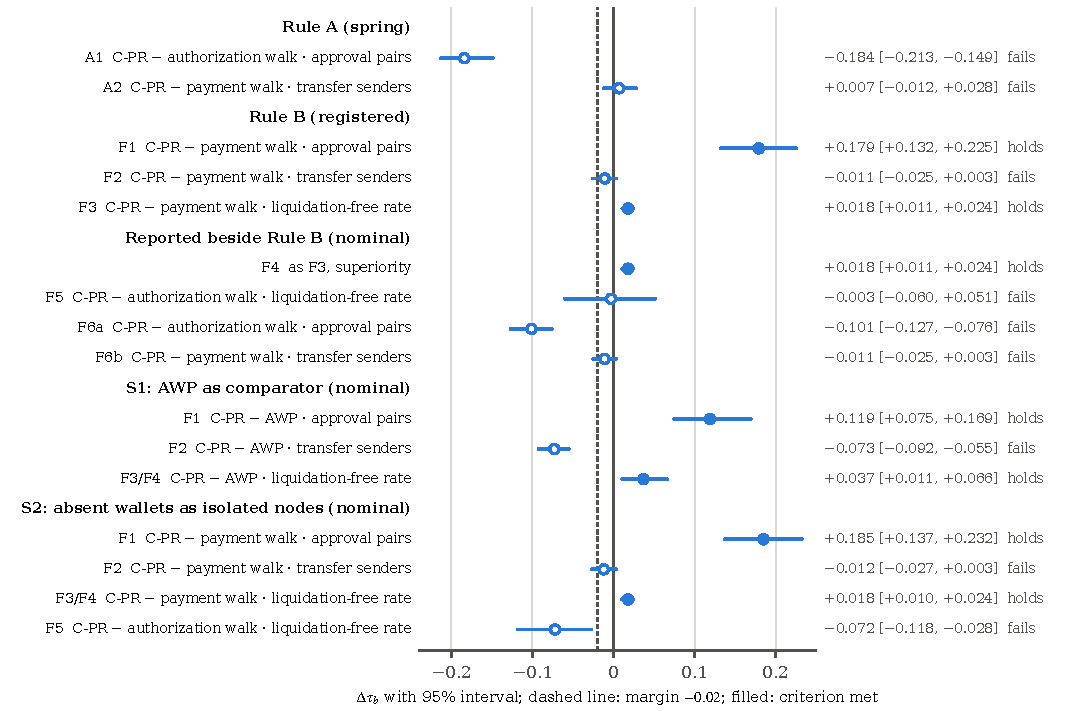
\includegraphics[width=\textwidth]{figures/fig_contrasts.pdf}
\caption{Contrasts fixed by Rules~A and~B and by the registered sensitivity analyses, with 95\% paired-bootstrap intervals (400 resamples, seed 42). Filled markers: criterion met; open markers: not met. The dashed line is the non-inferiority margin of $-0.02$. Only A1--A2 and F1--F3 decide a rule; the other verdicts are nominal and unadjusted.}
\label{fig:forest}
\end{figure*}

\subsection{Results Reported Beside the Decision}
These verdicts are nominal: each uses an unadjusted 95\% interval, and none was conditioned on another. F4 holds: on the liquidation-free close rate \cpr{} is ahead of the payment walk, not merely level with it. This is a pre-specified secondary result outside the failed rule, and the effect is small, as are all walk coefficients on this label (below 0.09). F5 fails, since \cpr{} and the authorization walk cannot be separated on that label ($-0.003$ $[-0.060,0.051]$). F6 fails on both parts, as in the spring: \cpr{} stays below the authorization walk on new approval pairs ($-0.101$ $[-0.127,-0.076]$) and is not above the payment walk on new senders.

Neither sensitivity analysis changes the decision. With AWP as the comparator (S1), F1 and F3 hold ($+0.119$ and $+0.037$), and F2 fails with its whole interval below the margin: AWP ranks new senders at 0.319, and \cpr{}'s deficit is $-0.073$ $[-0.092,-0.055]$. Against the published payment method, then, \cpr{} trades part of its ranking of later inflow for its gain on later approvals. With absent wallets kept as isolated nodes (S2), F1, F3 and F4 hold and F2 again fails ($-0.012$ $[-0.027,0.003]$). F5 changes from an unresolved difference to a deficit ($-0.072$ $[-0.118,-0.028]$) because the rule changes the ties of the authorization walk on the trader label. Of the 1,402 labeled traders, 41 score above the common value of addresses without approval in-edges, 1,278 sit at that value (three of them receive approvals whose share of their owners' rows is negligible under raw amounts), and 83 are absent from the authorization graph and score zero; the mean label values of the three groups are 1.000, 0.868 and 0.817. Under S2 the 83 absent traders join the large tie, the score becomes a two-level indicator of receiving approvals, and $\tau_b$, which divides by the number of pairs not tied on the score, rises from 0.086 to 0.155.

\subsection{The Weight Sweep}
\label{sec:sweep}
Fig.~\ref{fig:sweep} plots each label against $\lambda$, with the registered grid and four exploratory values near the end points. On new approval pairs the largest step comes at the lower end: switching the authorization layer on lifts \cpr{} from 0.044 to 0.271 in the spring and from 0.058 to 0.228 in the registered window, and most of that step is already present at $\lambda=0.01$ (0.217 and 0.203). At the upper end, $\lambda=0.99$ gives 0.327 and 0.245 against 0.479 and 0.338 at $\lambda=1$. Large steps thus come at both end points: at $\lambda=0$ every authorization row disappears, and at $\lambda=1$ the payment rows of wallets without authorization out-edges disappear. The F1 gain over the payment walk is a property of switching the authorization layer on, not of the value $\lambda=0.5$. On new transfer senders every interior value tested stays within 0.03 of the payment walk in both windows, while the authorization walk sits above it (0.372 against 0.270 in the spring, 0.289 against 0.257 in the registered window), probably because the spenders that many owners approve also attract many new payers (the in-approve degree reaches 0.404 and 0.371 on this label, Table~\ref{tab:holdout}). On the trader label the curve rises gently from 0.065 to 0.086.

Across the interior the ranking changes little even though the stationary distribution does not stand still. Between $\lambda=0.25$ and $0.75$ the $\ell_1$ distance between the two stationary vectors is 0.60 on the registered spender graph and 0.52 on the trader graph, and $r(B)$ falls from 0.46 to 0.42 and from 0.39 to 0.34; yet the Kendall $\tau$ between the two rankings of the cohort is 0.91 for spenders and 0.93 for traders. Proposition~\ref{prop:localize} therefore locates where the weight acts but does not explain why its effect on these rankings is small; the flat interior is an empirical finding of this sample.

\begin{figure*}[!t]
\centering
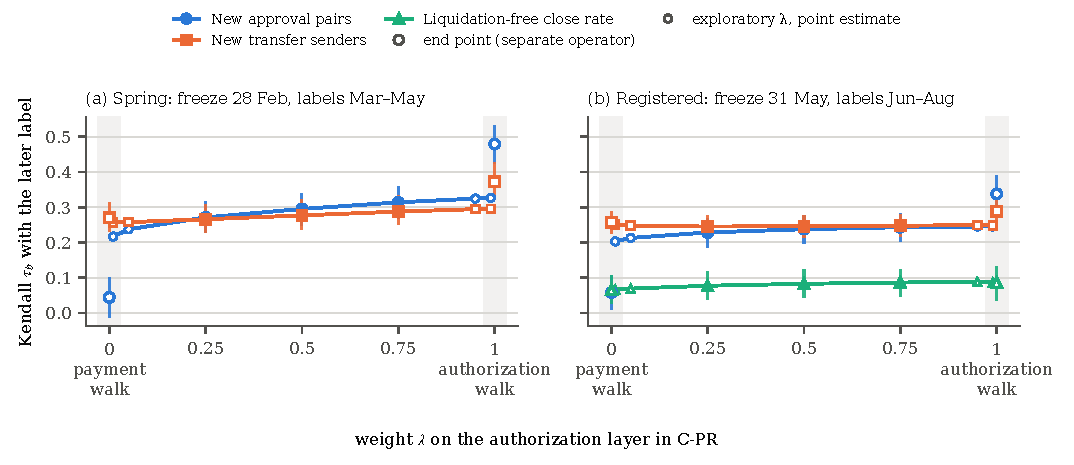
\includegraphics[width=\textwidth]{figures/fig_lambda_sweep.pdf}
\caption{Kendall $\tau_b$ of \cpr{} with each later label against the authorization weight $\lambda$. Filled markers with 95\% paired-bootstrap intervals are the registered grid $\lambda\in\{0.25,0.5,0.75\}$; open markers with intervals at $\lambda=0$ and $\lambda=1$ are the payment and authorization walks, separate operators that the line does not join; small open markers at $\lambda\in\{0.01,0.05,0.95,0.99\}$ are exploratory point estimates. (a) Spring holdout; the trader label was defined only for the registered window, so this panel has no trader curve. (b) Registered window. Values are in Table~\ref{tab:holdout} and Appendix~\ref{app:explore}.}
\label{fig:sweep}
\end{figure*}

\subsection{Seeded Restarts}
\spr{} reproduces the payment walk on new senders in both windows ($-0.006$ $[-0.017,0.006]$ in the spring and $-0.003$ $[-0.017,0.010]$ in the registered window). On new approval pairs it roughly doubles the payment walk's coefficient (0.114 against 0.044 in the spring, 0.126 against 0.058 in the registered window), yet it stays far below the authorization walk ($-0.365$ $[-0.431,-0.300]$ in the spring; 0.126 against 0.338 in the registered window, Table~\ref{tab:holdout}). It also trails the other walks on the trader label (0.030). Seeding thus moved the payment walk only part of the way toward the authorization signal. With $d=0.85$ only 15\% of the mass, plus the dangling mass, passes through the restart vector; at $d=0.5$ the seeded gain on new approval pairs barely changes ($+0.079$ and $+0.072$ over the payment walk at the same damping, against $+0.070$ and $+0.068$ at $d=0.85$; Appendix~\ref{app:explore}).

\subsection{Walks Against Counts, and a Decomposition}
No walk ranked either spender label as well as the raw count taken from that label's layer (Table~\ref{tab:holdout}). The in-approve degree reached 0.711 and 0.613 on new approval pairs; the authorization walk fell short by $-0.233$ $[-0.291,-0.183]$ in the spring, a contrast fixed with Rule~A, and EndorseRank by $-0.317$ $[-0.354,-0.283]$ and $-0.280$ $[-0.313,-0.247]$. The transfer in-degree reached 0.472 and 0.435 on new senders, ahead of AWP by $0.127$ $[0.099,0.150]$ and $0.116$ $[0.095,0.133]$. The companion study reports these reference comparisons in full \cite{KwonA2026}; they are repeated here because they bound what any walk in this paper can claim. On the trader label the in-approve degree at the freeze (0.144) also ranks above \cpr{} (\cpr{} minus the degree $-0.061$ $[-0.111,-0.011]$, post hoc). Most approval-receiving traders are contract accounts (40 of 44 in June to August), so account type is an unresolved confound of that count. Proposition~\ref{prop:closed} accounts for the authorization side: on a one-hop sample the walk is only a reweighted owner count, and on these arrival labels the reweighting lost accuracy. The degree result agrees with preferential attachment \cite{Barabasi1999,Newman2001} and with the strength of degree baselines in link prediction \cite{LibenNowell2007,Lin2022Tracking}.

\cpr{}'s registered lead over AWP on the trader label ($+0.037$) has two parts. The post hoc decomposition puts $+0.019$ $[-0.010,0.047]$ between the payment walk and AWP, which differ only in weights and restarts on the same transfers, and the remaining $+0.018$ is F4. By point estimates, about half of the registered lead over AWP thus comes from replacing AWP's bounded weights and activity restarts with raw amounts and uniform restarts rather than from authorization edges; that part is not resolved in June to August, where its interval includes zero, and is resolved in the spring ($+0.037$ $[0.011,0.063]$). Between the two layers walked alone the trader-label difference is unresolved in both windows. The companion study examines this label further at the level of counts \cite{KwonA2026}.

\subsection{Detectability}
The labels are sparse: 222 and 175 of the 1,335 spring spenders gained a new approval pair or a new payer, and 158 and 136 of the 1,964 registered spenders did, so each spender coefficient rests on how a small subset is ordered. Read as a binary outcome, the ranking quality is easier to picture: in the registered window the in-approve degree reaches an area under the receiver operating characteristic curve (AUC) of 0.93 for gaining an approval pair, the authorization walk 0.84, \cpr{} 0.80 and the payment walk 0.57; for gaining a new sender the transfer in-degree reaches 0.96 and \cpr{} 0.84 (Appendix~\ref{app:explore}). On the trader side 789 of the 1,402 traders had at least one liquidation, so that label is not sparse, but its coefficients are small, and passing F3 says little about practical value. F1 is large relative to its interval width and held again with a smaller point estimate. F2 is the narrow case. Its interval is 0.028 wide against 0.040 for the spring interval from which the margin was taken, so with this width a pass needed a point estimate above about $-0.006$. Its lower end lies $0.005$ beyond the margin. Across 50 further bootstrap seeds of 400 resamples, that endpoint has a standard deviation of 0.0008 and ranges from $-0.026$ to $-0.023$, so the miss is not resampling noise. The registered resample count and the verdict stand: F2 is a narrow failure against the payment walk and a clear one against AWP.

% =====================================================================
\section{Sybil Exposure of the Authorization Layer}
\label{sec:sybil}

The results above concern honest data. A reputation layer must also be judged by what it costs to fake. This section calibrates the farm results of Gy\"{o}ngyi and Garcia-Molina \cite{Gyongyi2005Alliances} to the authorization layer walked with uniform restarts, as in EndorseRank and in \cpr{} at $\lambda=1$, and then runs the same attacks on the other walks. The multipliers it reports depend on the sampled graph, in particular on how much mass the honest nodes concentrate, and would differ on a full graph.

\subsection{Cost of an Edge}
Approving a spender reserves nothing: no tokens are locked, and the approving address may hold a zero balance of that token. Under bounded weights an approval of a few base units weighs almost as much as an unlimited one, and after row normalization a single out-edge carries the whole row whatever its amount. An edge between two attacker addresses therefore exposes nothing and costs only gas. Because the score reads only approvals emitted inside its window, the attacker must re-emit each edge in every window it wants to keep, so over $q$ score refreshes a closed farm costs
\begin{equation}
C=q\,\bigl(|E_{\mathcal S}|\,c_{\text{gas}}+c_{\text{rev}}\bigr),
\label{eq:cost}
\end{equation}
where $c_{\text{gas}}$ is the fee of one approval and $c_{\text{rev}}$ a per-window allowance for revocations or detection avoidance. We did not measure $c_{\text{gas}}$; whatever its value, the cost is linear in edges and windows. A transfer of one base unit between farm addresses costs the same order of gas, so the edge itself is not cheaper in the authorization layer; what differs between layers is the score that the edge buys, as the computations below show.

\subsection{What a Closed Farm Collects}
Let every node of a farm $\mathcal S$ have out-edges, all inside $\mathcal S$, and let no honest owner approve a farm address. Write $r_D$ for the stationary mass on dangling nodes, all of which are honest. Summing (\ref{eq:pr}) over $\mathcal S$ with uniform $\boldsymbol\pi$ gives
\begin{equation}
\sum_{i\in\mathcal S} r_i=\frac{|\mathcal S|}{|V|}\cdot\frac{1-d+d\,r_D}{1-d}\le\frac{|\mathcal S|}{(1-d)|V|+d|\mathcal S|},
\label{eq:farm}
\end{equation}
where the bound uses $r_D\le 1-\sum_{i\in\mathcal S}r_i$. The second factor is the multiple of its population share that the farm captures, and it exceeds one whenever dangling nodes exist, because their redistributed mass reaches the farm. The bounded-weight authorization graph of our sample is dominated by dangling spenders: $r_D=0.532$, $0.553$ and $0.572$ at $d=0.75$, $0.85$ and $0.95$, so a closed farm captures 2.6, 4.1 and 11.9 times its population share. A ring of 20 addresses, each approving its successor, inserted into that graph captures 4.09 times its share at $d=0.85$.

The bound limits a farm's total mass, but the attacker can concentrate it. In a star, $m$ farm addresses each approve a target $t$ and $t$ approves each of them back. With $b=(1-d+d\,r_D)/|V|$, the mass each node receives from jumps and dangling rows, the balance equations give
\begin{equation}
r_t=\frac{b\,(1+d\,m)}{1-d^{2}}.
\label{eq:star}
\end{equation}
On the end-of-window EndorseRank graph $b=9.62\times10^{-5}$, the common score of every wallet that receives no approval. Take $m=10$, so that eleven addresses issue twenty approvals per window. On the augmented graph the target's score is $3.27\times10^{-3}$, which is 7.7 times the largest EndorseRank of any of the 5,521 sampled traders, and every further farm address adds $d\,b/(1-d^2)$ at the price of two more approvals per window. The comparison flatters the attack, because the sampled traders are mostly owners that sit at the floor $b$. The highest-scoring spender on the same graph scores 0.198, and the star reaches 1.7\% of it.

\subsection{The Same Farms on the Other Walks}
On AWP's graph, with bounded weights and activity restarts, a star of ten farm addresses that pay the target one base unit each and receive one back reaches $1.0\times10^{-4}$, 0.24\% of the largest AWP score among the sampled traders, and a ring of 20 collects 0.31 times its population share: activity restarts give each farm address the restart weight of one recent recipient, far below that of active honest senders. A farm that paid many recipients would raise its own restart weight, but a small farm gains little. In \cpr{} at $\lambda=0.5$, the renormalization in (\ref{eq:alpha}) lets a farm whose addresses approve only one another and make no payments follow its own edges with weight one, so the farm is closed exactly as in the authorization walk. Computed on the union graph of the trader cohort, a ring of 20 collects 2.44 times its share, and an authorization-only star lifts its target to 1.8\% of the largest \cpr{} score among the sampled traders. Coupling thus keeps the closed-farm gain of the authorization layer, while the denser payment layer raises the scores a farm must overtake.

Raw amounts change which approvals an attacker would buy from honest owners, not the closed-farm argument: in the raw-amount layer a bought approval moves much mass only if it is unlimited, and an unlimited approval hands the attacker the owner's entire balance of the token.

\subsection{Remedy, Untested}
The asymmetry that Cheng and Friedman identify points to the fix \cite{Cheng2005}. When jumps and the mass of dangling nodes are confined to a vetted seed set, as in TrustRank \cite{Gyongyi2004TrustRank}, a farm outside the seeds gains mass only along edges from honest owners, and those edges must be bought. We did not evaluate seeded restarts, and \spr{} is not such a remedy, because its seeds are authorization scores that a farm can inflate. Credential gates such as Human Passport \cite{HumanPassport} address a different question, whether an address belongs to a distinct person, and carry their own weaknesses \cite{Bordeianu2026}. The analysis is model-based and was checked with the solver on the observed graphs; no attack was run on chain.

% =====================================================================
\section{Threats to Validity}
\label{sec:threats}

\subsection{Construct Validity}
The spender labels are arrivals of the same kinds of edge that build the layers, counted on events with a sampled trader at one end, so they measure future attachment inside the trader-centered ego network and favor scores that track current counts. Neither is a credit or loss outcome. Most spenders are contracts (1,174 of 1,335 in the spring), so spender results concern routers, vaults and similar contracts more than people. The trader label is the nearest outcome to default in these data, but forced liquidation on one exchange is not default on a loan. The authorization edge is the latest in-window approval, not the allowance in force (Section~\ref{sec:model}). With the history cut to March--May, 15.8\% of the June--August pairs that would look new were allowances already held at the freeze. Allowances granted before December cannot be checked with our extraction, so some pairs counted as new are probably old relationships re-emitted; reading each allowance from contract state at the freeze block would settle the share. Permit2 takes 1,532 of the 21,585 latest allowances at the end of the window and 164 of the 2,168 registered approval-pair events. Zero-amount transfers, which include ERC-721 transfers, are 4.5\% of transfer logs and account for 5 of the 1,286 registered new-sender events. The raw-amount layers of \cpr{} let unlimited approvals and high-decimal tokens dominate rows; the exploratory reruns with bounded and binary weights show that the payment-side verdict depends on this choice.

\subsection{Internal Validity}
Rule~A was fixed after the spring results of its two comparators were known, and its precedence over the coupled scores is documented by a dated plan, not by a commit. Rule~B's hypothesis came from an exploratory spring contrast, and its margin came from the spring interval. The spring sample was selected partly on activity inside the spring label window, while the registered sample was not, and the score history doubled from 90 to 182 days between the windows; the spring rerun on a sample selected from December to February gives nearly the same contrasts. Rule~B's registration is a commit in the authors' own repository, not an entry in an independent registry; commit order, the server-side push times and the hashes in the extraction manifest become checkable once the repository is public, and a third-party timestamp would give a stronger guarantee. EndorseRank, the decomposition and the appendix analyses were computed outside the rules and are labeled accordingly. The rule that scores absent wallets as zero is a pipeline choice; sensitivity S2 shows that it changes F5 through the tie structure but no part of the decision.

\subsection{Statistical Conclusion Validity}
Rule-bound intervals come from 400 paired resamples, as registered; F2 misses the margin by 0.005 against the payment walk, about six Monte Carlo standard deviations of its endpoint, and by a wide margin against AWP. The decision is an intersection of three conditions, so no multiplicity correction applies to it, but the many contrasts reported beside it are nominal and should not be read as a family of tests. The wallet bootstrap treats spenders as independent although one new owner can approve several spenders. A two-way bootstrap that also reweights the owners or senders generating the label events changes the F1 and F2 intervals only slightly, to $[0.126,0.219]$ and $[-0.026,0.005]$, and a bootstrap over traders and calendar weeks gives $[0.009,0.025]$ for F3 and F4.

\subsection{External Validity}
The evidence comes from one rollup, one exchange's traders and their counterparties, nine months of logs and one-hop ego networks. Deeper samples, in which endorsements can travel more than one step, could behave differently, and the payment layer's density relative to the authorization layer may differ on other chains. Only fixed global weights with uniform teleportation were tested in the rules; node-dependent or learned weights, mixtures of stationary vectors, interlayer copies of nodes and per-layer damping remain open.

% =====================================================================
\section{Implications for Lending and Margin Protocols}
\label{sec:implications}

A protocol that screens counterparties or sets risk parameters from on-chain relations \cite{Bartoletti2021Lending,Perez2021Liquidations} can take four practical points from these results. First, on this sample the cheapest score was the best one: counting the distinct owners that approve an address anticipated its later approvals better than any walk, and counting distinct senders did the same for later payments, with no solver and no restart vector to defend. Second, mixing an authorization layer into a payment walk changed the ranking mainly by switching the authorization layer on, and the gain on later approvals came with an unresolved loss on later payments; a protocol that wants both signals can report the two counts side by side rather than fold them into one stationary distribution. Third, any score that walks authorization edges with uniform restarts can be inflated by a closed farm at the cost of gas alone, and the inflation is largest exactly where honest scores are low, as for ordinary wallets that receive few approvals. Restricting restarts to vetted seeds, or gating addresses before ranking them, is a precondition for using such a score in counterparty screening. Finally, approval logs are not allowance state: a protocol that acts on allowances should read them from contract state at the decision block rather than reconstruct them from a window of events.

% =====================================================================
\section{Conclusion}
\label{sec:conclusion}

Authorization and payment give two readings of the same wallets, and on this sample a walk that blends them at every wallet did not improve on the better of the two. Under the rule dated before any coupled score existed, \cpr{} trailed the authorization walk on later approvals and did not beat the payment walk on later senders. Under the rule registered before its data were extracted, it repeated its gain over the payment walk on later approvals and, as a pre-specified secondary result outside the rule, ranked later liquidation-free trading slightly better ($+0.018$ $[0.011,0.024]$, with every walk coefficient on that label below 0.09); but it could not be bounded within the registered margin on later transfer senders, so the rule is not met, and against AWP the loss on that label exceeded the margin. The gain on approvals appears as soon as the authorization layer is switched on and changes little across interior weights. Seeding the payment walk with authorization scores recovered only part of the authorization signal. On every spender label the raw degree of the label's layer outranked every walk, and on a one-hop sample the authorization walk is a reweighted count. Exploratory reruns show that the payment-side verdict depends on the raw-amount weighting, so the negative result concerns this operator on this sample rather than coupling in general. The authorization layer is also cheap to inflate under uniform restarts, and coupling does not remove that exposure. Future work should fix in advance, and test on unextracted data, couplings with comparable weights on both layers, samples deep enough for multi-hop propagation, and seed-restricted restarts under explicit attack.

% =====================================================================
\appendices
\section{Exploratory Checks}
\label{app:explore}

All checks below were run on 9 October 2026, after every registered and post hoc result was known, by the script in the supplement, which reuses the evaluation code unchanged and reproduces the registered scores exactly (largest absolute difference zero). None of them enters a rule. Table~\ref{tab:explore} lists the contrasts; the text adds the remaining diagnostics.

% Table 4: exploratory checks, run on 9 October 2026 after every result was known.
% Source: supplement/exploratory_checks.json (script supplement/exploratory_checks.py).
\begin{table*}[!t]
\centering
\caption{Exploratory Checks: Paired Contrasts $\Delta\tau=\tau_a-\tau_b$ Under Changes That No Rule Fixed}
\label{tab:explore}
\footnotesize
\setlength{\tabcolsep}{4pt}
\begin{tabular}{@{}lllcc@{}}
\toprule
Check & Contrast ($a$ minus $b$) & Label & Spring [95\% CI] & Registered [95\% CI] \\
\midrule
\multicolumn{5}{@{}l}{\emph{Spring sample selected from December--February closes only (1,170 spenders)}} \\
 & A1: C-PR minus C-PR ($\lambda=1$) & new approval pairs & $-$0.172 [$-$0.207, $-$0.142] & --- \\
 & A2: C-PR minus C-PR ($\lambda=0$) & new transfer senders & +0.014 [$-$0.006, 0.035] & --- \\
 & C-PR minus C-PR ($\lambda=0$) & new approval pairs & +0.251 [0.199, 0.300] & --- \\
\midrule
\multicolumn{5}{@{}l}{\emph{Both layers with bounded weights (EndorseRank's and AWP's), uniform restarts}} \\
 & C-PR minus C-PR ($\lambda=0$) & new approval pairs & +0.258 [0.203, 0.313] & +0.213 [0.168, 0.261] \\
 & C-PR minus C-PR ($\lambda=0$) & new transfer senders & $-$0.026 [$-$0.047, $-$0.005] & $-$0.010 [$-$0.022, 0.002] \\
 & C-PR minus C-PR ($\lambda=0$) & liquidation-free close rate & --- & +0.035 [0.025, 0.046] \\
 & C-PR minus C-PR ($\lambda=1$) & new approval pairs & $-$0.067 [$-$0.088, $-$0.045] & $-$0.061 [$-$0.080, $-$0.043] \\
\midrule
\multicolumn{5}{@{}l}{\emph{Both layers with binary weights, uniform restarts}} \\
 & C-PR minus C-PR ($\lambda=0$) & new approval pairs & +0.249 [0.196, 0.304] & +0.196 [0.151, 0.243] \\
 & C-PR minus C-PR ($\lambda=0$) & new transfer senders & +0.007 [$-$0.013, 0.027] & $-$0.006 [$-$0.017, 0.008] \\
 & C-PR minus C-PR ($\lambda=0$) & liquidation-free close rate & --- & +0.023 [0.014, 0.033] \\
 & C-PR minus C-PR ($\lambda=1$) & new approval pairs & $-$0.077 [$-$0.102, $-$0.052] & $-$0.058 [$-$0.078, $-$0.040] \\
\midrule
\multicolumn{5}{@{}l}{\emph{Registered operator, two-way bootstrap (spenders with label-generating owners or senders; traders with calendar weeks)}} \\
 & A1 / F6a: C-PR minus C-PR ($\lambda=1$) & new approval pairs & $-$0.184 [$-$0.206, $-$0.135] & --- \\
 & A2 / F2: C-PR minus C-PR ($\lambda=0$) & new transfer senders & +0.007 [$-$0.014, 0.024] & $-$0.011 [$-$0.026, 0.005] \\
 & F1: C-PR minus C-PR ($\lambda=0$) & new approval pairs & --- & +0.179 [0.126, 0.219] \\
 & F3: C-PR minus C-PR ($\lambda=0$) & liquidation-free close rate & --- & +0.018 [0.009, 0.025] \\
\midrule
\multicolumn{5}{@{}l}{\emph{Seeded ablation at $d=0.5$, against the payment walk at the same damping}} \\
 & S-PR minus C-PR ($\lambda=0$) & new approval pairs & +0.079 [0.050, 0.111] & +0.072 [0.045, 0.099] \\
 & S-PR minus C-PR ($\lambda=0$) & new transfer senders & $-$0.001 [$-$0.014, 0.014] & $-$0.004 [$-$0.021, 0.011] \\
\bottomrule
\end{tabular}

\vspace{2pt}
\parbox{\textwidth}{\footnotesize C-PR without a $\lambda$ is $\lambda=0.5$. Intervals: 400 paired resamples, seed 42, as in the registered analysis; the two-way rows add Poisson(1) weights on owners or senders, or a multinomial draw of the 14 weeks of the label window. Several variants were computed after the outcomes were known, so no row supports a claim on its own.}
\end{table*}


\emph{Look-ahead in the spring sample.} Restricting the sample to the 3,937 traders with at least three closes by 28 February, and keeping only the extracted events that touch one of them, leaves 1,170 spring spenders. On them A1 and A2 fail as before and the exploratory gain over the payment walk on new approval pairs is unchanged at $+0.251$ (Table~\ref{tab:explore}).

\emph{Edge weights.} Coupling the two layers with EndorseRank's and AWP's bounded weights under uniform restarts, or with binary weights, leaves the qualitative picture on approvals: \cpr{} gains on the payment walk and stays below the authorization walk. The payment-side contrast is what moves. With bounded weights its registered lower end is $-0.022$, just beyond the margin; with binary weights it is $-0.017$, inside it, so under binary weights all three registered contrasts would have met their criteria. In the spring, bounded weights make the coupled walk worse than the payment walk on new senders ($-0.026$ $[-0.047,-0.005]$). Several variants were tried after the outcomes were known, so these numbers locate the sensitivity of the result rather than rescue or condemn the coupling.

\emph{End points and interior.} At $\lambda\in\{0.01,0.05,0.95,0.99\}$, \cpr{} scores 0.217, 0.237, 0.324 and 0.327 on spring new approval pairs and 0.203, 0.213, 0.245 and 0.245 on registered ones; on new senders the registered values are 0.251, 0.248, 0.249 and 0.248, and on the trader label 0.066, 0.069, 0.088 and 0.086. The mass on $B$ is 0.44 on both spender graphs and 0.36 on the trader graph at $\lambda=0.5$.

\emph{AUC.} For gaining at least one new approval pair, the AUC difference between \cpr{} and the payment walk is $+0.229$ $[0.186,0.277]$ in the spring and $+0.228$ $[0.172,0.286]$ in the registered window; for gaining a new sender it is $+0.011$ $[-0.008,0.032]$ and $-0.011$ $[-0.030,0.009]$. These mirror the $\tau_b$ contrasts.

\emph{Precision and dependence.} Over 50 further seeds, the standard deviation of the lower endpoint is 0.0019 for A1, 0.0012 for A2, 0.0031 for F1, 0.0008 for F2 and 0.0004 for F3. The two-way bootstraps reweight, with Poisson(1) weights, the 1,206 owners and 894 senders that generate the registered label events alongside the spenders, and for F3 resample 14 calendar weeks of closes alongside the traders.

\emph{Parameters.} With $d=0.75$ or $0.95$, F1, F2 and F3 become $+0.180$, $-0.011$ $[-0.025,0.004]$ and $+0.015$, or $+0.178$, $-0.011$ $[-0.025,0.003]$ and $+0.022$; changing $k$ to 0.005 or 0.02, or $t_0$ to 90 or 270 days, moves no contrast by more than 0.001.

\emph{Edge diagnostics.} Of 617,098 approval logs, 48,857 carry value zero (revocations and ERC-721 approvals). Of 3,815,011 transfer logs, 170,209 carry value zero, 49,777 are mints from the zero address, 26,037 are burns to it and 200 are self-transfers; no registered new-sender event comes from the zero address. Permit2 receives 1,532 latest allowances from 816 owners at the end of the window and 335 of the 5,353 spring approval-pair events.

% =====================================================================
\section*{Acknowledgment}
The authors thank the School of Computing at the University of South Africa for supporting the first author's doctoral research, of which this study is part. The event logs were drawn from the public Arbitrum One dataset hosted on Google BigQuery; the queries cost less than USD~20. During the preparation of this work the authors used Claude (Anthropic) in order to assist with language editing, restructuring and checking of the text and analysis scripts. After using this tool, the authors reviewed and edited the content as needed and take full responsibility for the content of the published article.

\section*{Author Contributions}
Taehong Kwon: conceptualization, methodology, software, data curation, formal analysis, writing -- original draft. Ernest Mnkandla: supervision, writing -- review \& editing. Donatien Koulla Moulla: supervision, writing -- review \& editing. David Sena Attipoe: supervision, writing -- review \& editing.

\section*{Conflict of Interest}
The authors declare that they have no known competing financial interests or personal relationships that could have appeared to influence the work reported in this paper.

\section*{Data Availability}
The study uses only public blockchain data and involves no human participants. The code, configuration, registration files, extraction manifests, extracted logs and machine-readable result summaries are in the public repository \url{https://github.com/abitocodes/phd_works} (folder \path{1-Dissertation-Works/ERC20-Allowance-PageRank-Wallet-Reputation/dissertation/wallet-reputation-experiments}); the commits cited in Section~\ref{sec:gate} identify the registered state, and the evaluation code is at revision \sha{7129981}. The exploratory checks, the extraction queries and this manuscript's source are in \url{https://github.com/abitocodes/phd-dissertation-draft-en} (folder \path{manuscripts/B-ieee-access}). The supplement to this paper contains the extraction queries and the script and output of the exploratory checks. The repositories hold addresses only as they appear on the public ledger; no off-chain identity was collected or linked, and the paper reports aggregate results only.

\bibliographystyle{IEEEtran}
\bibliography{references}

\begin{IEEEbiographynophoto}{Taehong Kwon} is a Ph.D. candidate in computer science with the School of Computing, University of South Africa, Johannesburg, South Africa. Research interests include on-chain reputation, decentralized finance and graph-based ranking.
\end{IEEEbiographynophoto}

\begin{IEEEbiographynophoto}{Ernest Mnkandla} is a Professor with the School of Computing, University of South Africa, Johannesburg, South Africa. Research interests include software engineering and artificial intelligence.
\end{IEEEbiographynophoto}

\begin{IEEEbiographynophoto}{Donatien Koulla Moulla} is with the Centre for Augmented Intelligence and Data Science (CAIDS), School of Computing, University of South Africa, Johannesburg, South Africa.
\end{IEEEbiographynophoto}

\begin{IEEEbiographynophoto}{David Sena Attipoe} is with the Centre for Augmented Intelligence and Data Science (CAIDS), School of Computing, University of South Africa, Johannesburg, South Africa.
\end{IEEEbiographynophoto}

\EOD

\end{document}
